\section{引言}
\begin{frame}
  \frametitle{引言 | 基因组注释}
  \begin{block}{基因组注释(genome annotation)}
    从原始的基因组核酸序列中挖掘有用的生物学信息并阐释其生物学含义,包括基因组结构注释和基因组功能注释两大部分。
  \end{block}
  \pause
  \begin{block}{基因组结构注释(structural annotation)}
    在基因组序列中寻找基因等功能元件并明确其基本结构。
  \end{block}
  \pause
  \begin{block}{基因组功能注释(functional annotation)}
    在结构注释的基础上,将进化保守性(evolutionary conservation)和基因本体论(gene ontology)等元数据(meta-data)与功能元件对应起来,找到其生物学功能。
  \end{block}
\end{frame}

\begin{frame}
  \frametitle{引言 | 基因组注释}
  \begin{block}{基因组注释}
    \begin{itemize}
      \item 结构注释 $\Leftarrow$ 实验手段,单个基因
      \begin{itemize}
        \item 限制性酶切位点分析、开放阅读框分析、启动子分析、CpG岛识别
        \item 重复序列分析、基因识别
        \item mRNA选择性剪接分析
      \end{itemize}
      \item 功能注释 $\Leftarrow$ 组学时代,复杂疾病
      \begin{itemize}
        \item 变异位点的注释
        \item 基因集富集分析
        \item 生物学通路分析
        \item 相互作用网络分析
        \item 分子进化分析
      \end{itemize}
    \end{itemize}
  \end{block}
\end{frame}

\begin{frame}
  \frametitle{引言 | 基础知识}
  \begin{itemize}
    \item 基因组组装版本
    \item 基因组坐标系统
    \item 注释常用格式
    \item 文本编辑器
    \item 坐标的逻辑运算
  \end{itemize}
\end{frame}

\begin{frame}
  \frametitle{引言 | NGS}
  \begin{center}
    \includegraphics[width=10cm]{ngs.png}
  \end{center}
\end{frame}

\section{基因组组装版本}
\begin{frame}
  \frametitle{组装版本 | 疑惑}
  \begin{itemize}
    \item These sequences were mapped to human and mouse genomes sequences (\textcolor{blue}{hg18 and mm9}, respectively) using BLASTN.
    \item We used DNA sequences from the human and mouse genome assemblies \textcolor{blue}{hg18 and mm9}.
    \item Currently there are ~25,000 genes annotated in the human (\textcolor{blue}{hg18}) and mouse (\textcolor{blue}{mm9}) genome, which comprise less than 3\% of the genome (UCSC genome browser; http://genome.ucsc.edu/).
    \item The \textcolor{blue}{GRCh37/hg19 and GRCm38/mm10} assemblies at the UCSC genome browser (http://genome.ucsc.edu/) were used for mapping the chromosomal defect and gene annotations.
    \item The genome assemblies from which the sequences obtained were Dec 2011 (\textcolor{blue}{GRCm38/mm10}), Feb 2009 (\textcolor{blue}{GRCh37/hg19}) and Nov 2004 (\textcolor{blue}{Baylor3.4/rn4}) for mouse, human and rat respectively.
  \end{itemize}
\end{frame}


\begin{frame}
  \frametitle{组装版本 | XP vs. Win7}
  \begin{center}
    \includegraphics[width=9cm]{windows.png}
  \end{center}
\end{frame}

\begin{frame}
  \frametitle{组装版本 | \alert{版本对照}}
  \begin{center}
    \textcolor{blue}{基因组序列不是确定的吗?也需要版本升级?}
  \end{center}
  \pause
  \begin{table}
    \centering
    \rowcolors[]{1}{blue!20}{blue!10}
    \begin{tabular}{cccc}
      \hline
      \rowcolor{blue!50} SPECIES & UCSC & DATE & NCBI\\
      Human & hg38 & Dec. 2013 & GRCh38\\
       & hg19 & Feb. 2009 & GRCh37\\
       & hg18 & Mar. 2006 & NCBI Build 36.1\\
       & hg17 & May 2004 & NCBI Build 35\\
       & hg16 & Jul. 2003 & NCBI Build 34\\
      \hline
      Mouse & mm10 & Dec. 2011 & GRCm38\\
       & mm9 & Jul. 2007 & NCBI Build 37\\
       & mm8 & Feb. 2006 & NCBI Build 36\\
       & mm7 & Aug. 2005 & NCBI Build 35\\
      \hline
    \end{tabular}
  \end{table}
  \pause
  \begin{center}
    human: \textit{Homo sapiens}; mouse: \textit{\alert{M}us \alert{m}usculus}

    hg: \alert{h}uman \alert{g}enome; GRC: \alert{G}enome \alert{R}eference \alert{C}onsortium
  \end{center}
\end{frame}

\begin{frame}
  \frametitle{组装版本 | \textcolor{gray}{坐标转换}}
  \begin{itemize}
    \item \href{http://genome.ucsc.edu/cgi-bin/hgLiftOver}{UCSC liftOver tool}:支持BED和“chrN:start-end”格式的输入
    \item \href{https://usegalaxy.org/}{Galaxy(基于UCSC liftOver tool)}:支持BED、GFF和GTF格式的输入
    \item \href{http://crossmap.sourceforge.net/}{CrossMap}:支持SAM/BAM、Wiggle/BigWig、BED、GFF/GTF和VCF格式的输入,输出对应格式
    \item \href{http://www.ncbi.nlm.nih.gov/genome/tools/remap}{NCBI Remap}:支持BED、GFF、GTF和VCF等格式的输入
    \item \href{http://asia.ensembl.org/Homo\_sapiens/UserData/SelectFeatures}{\textcolor{gray}{Ensembl assembly converter(2015年退休,CrossMap继位)}}\textcolor{gray}{:支持BED、GFF、GFT和PSL格式的输入,但输出都是GFF格式的}
    \item \href{https://pypi.python.org/pypi/pyliftover}{pyliftover}:仅支持点坐标(point coordinates)的转换,无法对区段(ranges)坐标进行转换
  \end{itemize}
\end{frame}

\section{基因组坐标系统}
\begin{frame}
  \frametitle{坐标系统 | 坐标轴}
  \only<1,2>{
  \begin{center}
    \includegraphics[width=6cm]{2d.png}
  \end{center}
  }
  \pause
  \only<2,3>{
  \begin{center}
    \includegraphics[width=9cm]{1d.png}
  \end{center}
  }
  \pause
  \only<3,4>{
  \begin{center}
    \includegraphics[width=7cm]{dna.png}
  \end{center}
  }
  \pause
  \only<4>{
  \begin{block}{hg19}
    \begin{itemize}
      \item SNP, rs1800468: ``chr19\ \ \ 41860587''; ``chr19:41860587''
      \item gene, \textit{SAMD11}: ``chr1 \ \ \ 861121\ \ \ 879961''; ``chr1:861121-879961''
    \end{itemize}
  \end{block}
  }
\end{frame}

\begin{frame}
  \frametitle{坐标系统 | \alert{两大系统}}
  \begin{block}{序列}
  \begin{table}
    \centering
    \rowcolors[]{1}{blue!20}{blue!10}
    \begin{tabular}{lcccccccc}
      \hline
      0-based index & 0 & 1 & 2 & 3 & 4 & 5 & 6 & 7\\
      \hline
      Sequence & A & A & T & T & G & G & C & C\\
      \hline
      1-based index & 1 & 2 & 3 & 4 & 5 & 6 & 7 & 8\\
      \hline
    \end{tabular}
  \end{table}
  \end{block}
  \pause
  \begin{block}{TG的坐标}
    \begin{itemize}
      \item 0-based,half-open:[3,5)
      \item 1-based,fully-closed:[4,5]
    \end{itemize}
  \end{block}
  \pause
  \begin{block}{实例}
    \begin{itemize}
      \item 0-based:BED、BAM、PSL,dbSNP、Table Browser
      \item 1-based:GFF、VCF、SAM、Wiggle,DAS、Genome Browser
    \end{itemize}
  \end{block}
\end{frame}

\begin{frame}
  \frametitle{坐标系统 | 类比}
  \begin{columns}
  \column{0.5\textwidth}
  \visible<1->{
  \begin{block}{first floor}
    \begin{center}
      \includegraphics[width=6cm]{firstFloor.png}
    \end{center}
  \end{block}
  }
  \column{0.48\textwidth}
  \visible<2->{
  \begin{block}{数组}
    \begin{center}
      \includegraphics[width=5.5cm]{array.png}
    \end{center}
  \end{block}
  }
  \end{columns}
\end{frame}

\section{基因组注释常用格式}
\begin{frame}
  \frametitle{格式 | 文件格式}
    \begin{center}
      \includegraphics[width=7cm]{format.jpg}
    \end{center}
\end{frame}

\begin{frame}
  \frametitle{格式 | FASTA}
    \begin{center}
      \includegraphics[width=12cm]{fasta.png}
    \end{center}
\end{frame}

\begin{frame}
  \frametitle{格式 | FASTA | 注意事项}
  \begin{itemize}
    \item 每一行最好不要超过80个字符
    \item 序列中的换行符不会影响序列的连续性
    \item 使用标准的IUB/IUPAC核酸代码和氨基酸代码
    \item 允许小写字母的存在,但会转换成大写
    \item 单个“-”代表不明长度的空位
    \item 在氨基酸序列中允许出现“U”和“*”
    \item 任何数字都应该被去掉或转换成字母
    \item 不明核酸和氨基酸分别用“N”和“X”表示
  \end{itemize}
\end{frame}

\begin{frame}
  \frametitle{格式 | FASTA | IUB/IUPAC核酸}
    \begin{center}
      \includegraphics[width=8cm]{iub.png}
    \end{center}
\end{frame}

\begin{frame}
  \frametitle{格式 | FASTA | IUB/IUPAC核酸}
    \begin{center}
      \includegraphics[width=12cm]{na.png}
    \end{center}
\end{frame}

\begin{frame}
  \frametitle{格式 | FASTA | IUB/IUPAC氨基酸}
    \begin{center}
      \includegraphics[width=11cm]{aa.png}
    \end{center}
\end{frame}

\begin{frame}
  \frametitle{格式 | FASTA | FASTA vs. Sequence}
  \begin{block}{FASTA}
    \begin{center}
      \includegraphics[width=12cm,height=4cm]{fasta.png}
    \end{center}
  \end{block}
  \begin{block}{Sequence}
    \begin{itemize}
      \item {\scriptsize GTACGACGGAGTGTTATAAGATGGGAAATCGGATACCAGATGAAATTGTGGATCAG}
      \item {\scriptsize MWTALPLLCAGAWLLSAGATAELTVNAIEKFHFTSWMKQHQKTYSSREYSHRLQVFAN}
    \end{itemize}
  \end{block}
\end{frame}

\begin{frame}
  \frametitle{格式 | BED (Browser Extensible Data)}
    \begin{center}
      \includegraphics[width=12cm,height=5.5cm]{bed.png}
    \end{center}
\end{frame}

\begin{frame}
  \frametitle{格式 | \alert{BED\#}}
  \begin{block}{BED\#}
  \begin{description}
    \item[BED12]<alert@1> 包含全部12列
    \item[BED6]<alert@2> \alert{chrom, start, end, name, score, and strand}
    \item[BED5]<alert@3> chrom, start, end, name, and score
    \item[BED4]<alert@4> chrom, start, end, and name
    \item[BED3]<alert@5> chrom, start, and end
  \end{description}
\end{block}
\begin{block}{例子}
    \only<1>{chr1\ \ \ \ \ 11873\ \ \ \ \ 14409\ \ \ \ \ uc001aaa.3\ \ \ \ \ 0\ \ \ \ \ +\ \ \ \ \ 11873\ \ \ \ \ 11873\ \ \ \ \ 0\ \ \ \ \ 3\ \ \ \ \ 354,109,1189,\ \ \ \ \ 0,739,1347,}
    \only<2>{chr1\ \ \ \ \ 11873\ \ \ \ \ 14409\ \ \ \ \ uc001aaa.3\ \ \ \ \ 0\ \ \ \ \ +}
    \only<3>{chr1\ \ \ \ \ 11873\ \ \ \ \ 14409\ \ \ \ \ uc001aaa.3\ \ \ \ \ 0}
    \only<4>{chr1\ \ \ \ \ 11873\ \ \ \ \ 14409\ \ \ \ \ uc001aaa.3}
    \only<5>{chr1\ \ \ \ \ 11873\ \ \ \ \ 14409}
  \end{block}
\end{frame}

\begin{frame}
  \frametitle{格式 | GFF (General Feature Format)}
    \begin{center}
      \includegraphics[width=12cm,height=4.5cm]{gff.png}
    \end{center}
\end{frame}

\begin{frame}
  \frametitle{格式 | VCF (Variant Call Format)}
    \begin{center}
      \includegraphics[width=12cm,height=5.5cm]{vcf.png}
    \end{center}
\end{frame}

\section{文本文件与文本编辑器}
\begin{frame}
  \frametitle{文本 | 纯文本 vs. 格式化文本}
    \begin{center}
      \includegraphics[width=5.9cm,height=6.45cm]{txt.png}
      \vspace*{0.1cm}
      \includegraphics[width=6cm]{word.png}
    \end{center}
\end{frame}

\begin{frame}[fragile]
  \frametitle{文本 | 换行符}
  \begin{block}{三大类}
    \begin{itemize}
      \item Windows:\verb|\r\n|(CR+LF,回车+换行),文件尾部直接EOF(文件结束标志)
      \item Unix:\verb|\n|(LF,仅有换行),文件最后一行也会增加该字符,然后才是EOF
      \item \textcolor{gray}{Mac}:\verb|\r|(CR,仅有回车)
    \end{itemize}
  \end{block}
  \pause
  \begin{block}{识别与转换}
    \begin{itemize}
      \item Windows:文本编辑器,如Notepad++
      \item Unix:file识别,fromdos/todos或者dos2unix/unix2dos转换
    \end{itemize}
  \end{block}
\end{frame}

\begin{frame}
  \frametitle{文本 | 编辑器}
    \begin{center}
      \includegraphics[width=9cm]{editor.png}
    \end{center}
\end{frame}

\begin{frame}
  \frametitle{文本 | 编辑器 | Notepad++}
    \begin{center}
      \includegraphics[width=10cm]{notepad.png}
    \end{center}
\end{frame}

\begin{frame}
  \frametitle{文本 | 编辑器 | Vim}
    \begin{center}
      \includegraphics[width=10cm]{vim.jpg}
    \end{center}
\end{frame}

\begin{frame}
  \frametitle{文本 | 编辑器 | Emacs}
    \begin{center}
      \includegraphics[width=8cm]{emacs.png}
    \end{center}
\end{frame}

\begin{frame}
  \frametitle{文本 | 编辑器 | Sublime Text}
    \begin{center}
      \includegraphics[width=11cm]{sublime.png}
    \end{center}
\end{frame}

\begin{frame}
  \frametitle{文本 | 编辑器 | Atom}
    \begin{center}
      \includegraphics[width=11cm]{atom_01.png}
    \end{center}
\end{frame}

\section{基因组坐标的逻辑运算}
\begin{frame}
  \frametitle{逻辑运算 | 常见问题}
  \begin{block}{数据}
    \begin{description}
      \item[gene1] chr1 \quad 10 \quad 20 \quad +
      \item[gene2] chr1 \quad 40 \quad 60 \quad +
      \item[gene3] chr1 \quad 50 \quad 100 \quad +
      \item[snp1] chr1 \quad 15 \quad +
      \item[snp2] chr1 \quad 55 \quad -
      \item[exon3.1] chr1 \quad 50 \quad 60 \quad +
      \item[exon3.2] chr1 \quad 90 \quad 100 \quad +
    \end{description}
  \end{block}
  \vspace{-0.5em}
  \pause
  \begin{block}{问题}
    \begin{enumerate}
      \item 找到gene1和gene2之间的基因间区域。
      \item snp1在gene1上吗?snp2在gene1上吗(,在gene2上吗)?
      \item 找到与gene3重叠和不重叠的基因?
      \item 找到gene3的内含子区域。
    \end{enumerate}
  \end{block}
\end{frame}

\begin{frame}
  \frametitle{逻辑运算 | 集合运算}
    \begin{center}
      \includegraphics[width=9cm]{set.png}
    \end{center}
\end{frame}

\begin{frame}
  \frametitle{逻辑运算 | 集合 $\Rightarrow$ 基因组}
    \begin{center}
      \includegraphics[width=9cm]{setT.png}
    \end{center}
\end{frame}

\begin{frame}
  \frametitle{逻辑运算 | \alert{运算模式}}
    \begin{center}
      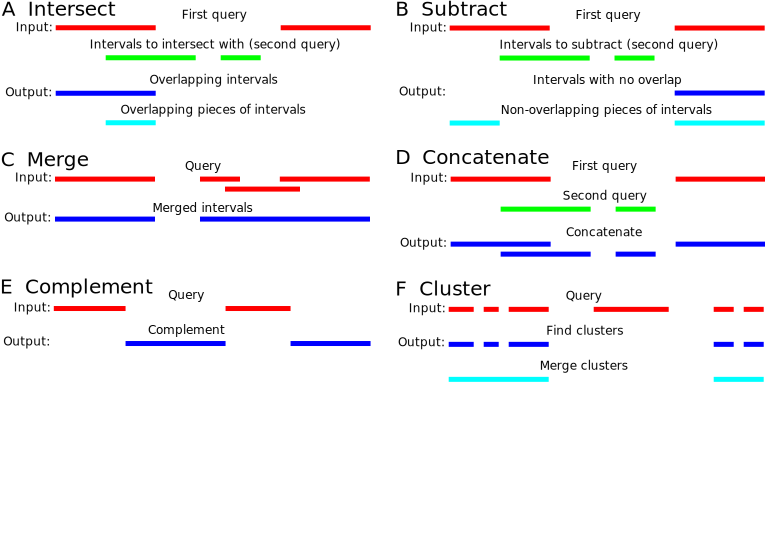
\includegraphics[width=11cm]{operation.png}
    \end{center}
\end{frame}

\begin{frame}
  \frametitle{逻辑运算 | intersect}
    \begin{center}
      \includegraphics[width=11cm]{intersect.png}
    \end{center}
\end{frame}

\begin{frame}
  \frametitle{逻辑运算 | intersect}
    \begin{center}
      \includegraphics[width=11cm]{intersectA.png}
      \vspace{0.5cm}
      \includegraphics[width=11cm]{intersectB.png}
    \end{center}
\end{frame}

\begin{frame}
  \frametitle{逻辑运算 | subtract}
    \begin{center}
      \includegraphics[width=11cm]{subtract.png}
    \end{center}
\end{frame}

\begin{frame}
  \frametitle{逻辑运算 | subtract}
    \begin{center}
      \includegraphics[width=11cm]{subtractA.png}
      \vspace{0.5cm}
      \includegraphics[width=11cm]{subtractB.png}
    \end{center}
\end{frame}

\begin{frame}
  \frametitle{逻辑运算 | merge}
    \begin{center}
      \includegraphics[width=11cm]{merge.png}
    \end{center}
\end{frame}

\begin{frame}
  \frametitle{逻辑运算 | merge}
    \begin{center}
      \includegraphics[width=11cm]{mergeA.png}
      \vspace{0.5cm}
      \includegraphics[width=11cm]{mergeB.png}
    \end{center}
\end{frame}

\begin{frame}
  \frametitle{逻辑运算 | concatenate}
    \begin{center}
      \includegraphics[width=11cm]{concatenate.png}
    \end{center}
\end{frame}

\begin{frame}
  \frametitle{逻辑运算 | complement}
    \begin{center}
      \includegraphics[width=11cm]{complement.png}
    \end{center}
\end{frame}

\begin{frame}
  \frametitle{逻辑运算 | complement}
    \begin{center}
      \includegraphics[width=11cm]{complementA.png}
      \vspace{0.5cm}
      \includegraphics[width=11cm]{complementB.png}
    \end{center}
\end{frame}

\begin{frame}
  \frametitle{逻辑运算 | cluster}
    \begin{center}
      \includegraphics[width=11cm]{cluster.png}
    \end{center}
\end{frame}

\begin{frame}
  \frametitle{逻辑运算 | cluster}
    \begin{center}
      \includegraphics[width=11cm]{clusterB.png}
    \end{center}
\end{frame}

\begin{frame}
  \frametitle{逻辑运算 | join}
    \begin{center}
      \includegraphics[width=12cm]{join1.png}
    \end{center}
\end{frame}

\begin{frame}
  \frametitle{逻辑运算 | join}
    \begin{center}
      \includegraphics[width=12cm]{join2.png}
    \end{center}
\end{frame}

\begin{frame}
  \frametitle{逻辑运算 | join}
    \begin{center}
      \includegraphics[width=12cm]{join3.png}
    \end{center}
\end{frame}

\begin{frame}
  \frametitle{逻辑运算 | join}
    \begin{center}
      \includegraphics[width=12cm]{join4.png}
    \end{center}
\end{frame}

\begin{frame}
  \frametitle{逻辑运算 | 其他}
  \begin{description}
    \item[coverage] Finds the number of bases each interval in the first dataset covers of the second dataset.
    \item[flank] Finds the upstream and/or downstream flanking region(s).
    \item[closest] Find the closest, potentially non-overlapping upstream and/or downstream features.
    \item[slop] Adjust the size of intervals.
    \item[window] Find overlapping intervals within a window around an interval.
  \end{description}
\end{frame}

\begin{frame}
  \frametitle{逻辑运算 | \alert{实例}}
  \begin{columns}
    \column{0.45\textwidth}
    \begin{block}{Dataset 1}
chr1\ \ \ 10\ \ \ \ \ 49\ \ \ \ \ Feature1.1\\
chr1\ \ \ 70\ \ \ \ \ 119\ \ \ Feature1.2\\
chr1\ \ \ 170\ \ \ 209\ \ \ Feature1.3\\
chr1\ \ \ 180\ \ \ 229\ \ \ Feature1.4
    \end{block}
    \column{0.45\textwidth}
    \begin{block}{Dataset 2}
chr1\ \ \ 80\ \ \ \ \ 109\ \ \ Feature2.1\\
chr1\ \ \ 150\ \ \ 199\ \ \ Feature2.2\\
chr1\ \ \ 250\ \ \ 289\ \ \ Feature2.3\\
chr1\ \ \ 270\ \ \ 309\ \ \  Feature2.4
    \end{block}
  \end{columns}
  \only<2>{
  \begin{block}{intersect}
chr1\ \ \ 80\ \ \ \ \ 109\ \ \ Feature3.1\\
chr1\ \ \ 170\ \ \ 199\ \ \ Feature3.2\\
chr1\ \ \ 180\ \ \ 199\ \ \ Feature3.3
  \end{block}
  }
  \only<3>{
  \begin{columns}
    \column{0.45\textwidth}
  \begin{block}{subtract (1-2)}
chr1\ \ \ 10\ \ \ \ \ 49\ \ \ \ \ Feature4.1\\
chr1\ \ \ 70\ \ \ \ \ 80\ \ \ \ \ Feature4.2\\
chr1\ \ \ 109\ \ \ 119\ \ \ Feature4.3\\
chr1\ \ \ 199\ \ \ 209\ \ \ Feature4.4\\
chr1\ \ \ 199\ \ \ 229\ \ \ Feature4.5
  \end{block}
  \column{0.45\textwidth}
  \begin{block}{subtract (2-1)}
chr1\ \ \ 150\ \ \ 170\ \ \ Feature5.1\\
chr1\ \ \ 250\ \ \ 289\ \ \ Feature5.2\\
chr1\ \ \ 270\ \ \ 309\ \ \ Feature5.3\\
\quad \\
\quad
  \end{block}
\end{columns}
  }
  \only<4>{
  \begin{block}{join}
chr1\ \ \ 70\ \ \ \ \ 119\ \ \ Feature1.2\qquad chr1\ \ \ 80\ \ \ \ \ 109\ \ \ Feature2.1\\
chr1\ \ \ 170\ \ \ 209\ \ \ Feature1.3\qquad chr1\ \ \ 150\ \ \ 199\ \ \ Feature2.2\\
chr1\ \ \ 180\ \ \ 229\ \ \ Feature1.4\qquad chr1\ \ \ 150\ \ \ 199\ \ \ Feature2.2
  \end{block}
  }
\end{frame}

\begin{frame}
  \frametitle{逻辑运算 | \alert{应用}}
  \begin{block}{实际问题}
  \begin{enumerate}
    \item Find genes that overlap LINEs.
    \item Remove introns from gene features. Exons will (should) be reported.
    \item Merge overlapping repetitive elements into a single entry.
    \item Report all intervals in the human genome that are not covered by repetitive elements.
  \end{enumerate}
\end{block}
  \pause
  \begin{block}{解决策略}
  \begin{enumerate}
    \item intersect
    \item subtract
    \item merge
    \item complement
  \end{enumerate}
\end{block}
\end{frame}

\begin{frame}
  \frametitle{逻辑运算 | 工具}
  \begin{itemize}
    \item \href{https://usegalaxy.org/}{Galaxy} 中的“Operate on Genomic Intervals”工具集
    \item \href{http://bedtools.readthedocs.org/en/latest/}{bedtools}: a powerful toolset for genome arithmetic
    \item \href{https://bedops.readthedocs.org/en/latest/}{BEDOPS}: the fast, highly scalable and easily-parallelizable genome analysis toolkit
  \end{itemize}
\end{frame}

\section{总结与答疑}
\begin{frame}
  \frametitle{总结与答疑}
  \begin{block}{知识点——基因组注释基础}
    \begin{itemize}
      \item 基因组组装版本——对应关系
      \item 两种坐标系统——0-based和1-based
      \item 四种常用格式——FASTA,BED,GFF,VCF
      \item 坐标逻辑运算——常见模式及其适用范围
      \item \textcolor{gray}{坐标转换、格式转换、}逻辑运算的工具
    \end{itemize}
  \end{block}
  \begin{block}{技能——纯文本与文本编辑器}
    \begin{itemize}
      \item 纯文本与格式化文本
      \item 不同操作系统中的换行符
      \item 文本编辑器——Notepad++,Vim,Emacs
    \end{itemize}
  \end{block}
\end{frame}
